\documentclass[fleqn]{article}
\usepackage{amsmath}
\usepackage[table]{xcolor}
\usepackage{graphicx}

\begin{document}
% top matter
\title{CS 6680 - Final Exam}
\author{Brendan Robeson}
\maketitle

\begin{description}

% problem 1.1 {{{
\item [1.1]
    \begin{math}p \oplus 3B =\end{math}

    \begin{tabular}{| c | c | c | c | c | c | c | c | c | c | c | c | c | c | c | c | c |}
        \hline
        & & & \cellcolor{gray} & \cellcolor{gray} & \cellcolor{gray} & \cellcolor{gray} & \cellcolor{gray} & \cellcolor{gray} & \cellcolor{gray} & & & & & & & \\ \hline
        & & & \cellcolor{gray} & \cellcolor{gray} & \cellcolor{gray} & \cellcolor{gray} & \cellcolor{gray} & \cellcolor{gray} & \cellcolor{gray} & & & & & & & \\ \hline
        & & & \cellcolor{gray} & \cellcolor{gray} & \cellcolor{gray} & \cellcolor{gray} & \cellcolor{gray} & \cellcolor{gray} & \cellcolor{gray} & & & & & & & \\ \hline
        & & & \cellcolor{gray} & \cellcolor{gray} & \cellcolor{gray} & \cellcolor{gray} & \cellcolor{gray} & \cellcolor{gray} & \cellcolor{gray} & & & & & & & \\ \hline
        & & & \cellcolor{gray} & \cellcolor{gray} & \cellcolor{gray} & \cellcolor{gray} & \cellcolor{gray} & \cellcolor{gray} & \cellcolor{gray} & & & & & & & \\ \hline
        & & & \cellcolor{gray} & \cellcolor{gray} & \cellcolor{gray} & \cellcolor{gray} & \cellcolor{gray} & \cellcolor{gray} & \cellcolor{gray} & & & & & & & \\ \hline
        & & & \cellcolor{gray} & \cellcolor{gray} & \cellcolor{gray} & \cellcolor{gray} & \cellcolor{gray} & \cellcolor{gray} & \cellcolor{gray} & & & & & & & \\ \hline
        & & & & & & & & & & & & & & & & \\ \hline
        & & & & & & & & & & & & & & & & \\ \hline
        & & & & & & & & & & & & & & & & \\ \hline
        & & & & & & & & & & & & & & & & \\ \hline
        & & & & & & & & & & & & & & & & \\ \hline
    \end{tabular}

    \begin{math}(p \oplus 3B) \cap A =\end{math}

    \begin{tabular}{| c | c | c | c | c | c | c | c | c | c | c | c | c | c | c | c | c |}
        \hline
        & & & & & & & & & & & & & & & & \\ \hline
        & & & & & & & & & & & & & & & & \\ \hline
        & & & \cellcolor{gray} & \cellcolor{gray} & \cellcolor{gray} & \cellcolor{gray} & \cellcolor{gray} & & & & & & & & & \\ \hline
        & & & \cellcolor{gray} & \cellcolor{gray} & \cellcolor{gray} & \cellcolor{gray} & \cellcolor{gray} & & & & & & & & & \\ \hline
        & & & \cellcolor{gray} & \cellcolor{gray} & \cellcolor{gray} & \cellcolor{gray} & \cellcolor{gray} & & & & & & & & & \\ \hline
        & & & & & \cellcolor{gray} & \cellcolor{gray} & \cellcolor{gray} & \cellcolor{gray} & \cellcolor{gray} & & & & & & & \\ \hline
        & & & \cellcolor{gray} & \cellcolor{gray} & \cellcolor{gray} & \cellcolor{gray} & \cellcolor{gray} & & & & & & & & & \\ \hline
        & & & & & & & & & & & & & & & & \\ \hline
        & & & & & & & & & & & & & & & & \\ \hline
        & & & & & & & & & & & & & & & & \\ \hline
        & & & & & & & & & & & & & & & & \\ \hline
        & & & & & & & & & & & & & & & & \\ \hline
    \end{tabular}
% }}}

% problem 1.2 {{{
\item [1.2]
    The geodetic distance is 5.
    \begin{displaymath}
        p1_x - p_x = 12 - 7 = 5
    \end{displaymath}
% }}}

% problem 1.3 {{{
\item [1.3] \begin{equation} A \oplus B \end{equation}
B is a disk structuring element of radius 8, with its origin at the center of
the disk.

\item [2.1.a]
\begin{displaymath}
T = \{ 3, 2, 2, 5, 2, 2 ,7, 7, 7, 6, 7, 8, 6, 7, 3, 4, 5 \}
\end{displaymath}
% }}}

% problem 2.1.a {{{
\item [2.1.a]
    In the data below, gray pixels must already be designated as border pixels. The green pixel is the next pixel to be added to region 1. The light gray pixels are new border pixels.

    \begin{tabular}{| c | c | c | c | c | c | c | c |}
        \hline
        3 & 2 & 2 & \cellcolor{orange} 1 & \cellcolor{orange} 1 & \cellcolor{orange} 1 & \cellcolor{orange} 1 & \cellcolor{orange} 1 \\ \hline
        \cellcolor{orange} 6 & 5 & \cellcolor{gray} 2 & \cellcolor{gray} 2 & \cellcolor{orange} 1 & \cellcolor{orange} 1 & \cellcolor{orange} 1 & \cellcolor{orange} 1 \\ \hline
        \cellcolor{orange} 7 & \cellcolor{orange} 7 & \cellcolor{orange} 7 & \cellcolor{gray} 7 & \cellcolor{lightgray} 7 & \cellcolor{orange} 1 & \cellcolor{orange} 1 & \cellcolor{orange} 1 \\ \hline
        \cellcolor{orange} 7 & \cellcolor{orange} 7 & \cellcolor{orange} 6 & \cellcolor{green} 7 & \cellcolor{lightgray} 6 & 7 & \cellcolor{orange} 1 & \cellcolor{orange} 1 \\ \hline
        \cellcolor{orange} 8 & \cellcolor{orange} 7 & \cellcolor{orange} 7 & \cellcolor{gray} 8 & \cellcolor{lightgray} 6 & 7 & \cellcolor{orange} 1 & \cellcolor{orange} 1 \\ \hline
        \cellcolor{orange} 8 & \cellcolor{orange} 8 & \cellcolor{orange} 7 & \cellcolor{gray} 3 & \cellcolor{orange} 2 & \cellcolor{orange} 1 & \cellcolor{orange} 1 & \cellcolor{orange} 1 \\ \hline
        \cellcolor{orange} 8 & \cellcolor{orange} 8 & \cellcolor{orange} 8 & \cellcolor{gray} 4 & \cellcolor{orange} 2 & \cellcolor{orange} 1 & \cellcolor{orange} 2 & \cellcolor{orange} 1 \\ \hline
        \cellcolor{orange} 8 & \cellcolor{orange} 8 & \cellcolor{orange} 8 & \cellcolor{gray} 5 & \cellcolor{orange} 1 & \cellcolor{orange} 1 & \cellcolor{orange} 1 & \cellcolor{orange} 1 \\ \hline
    \end{tabular}

    Using notation (x,y)...
    \begin{align*}
        \mu_1 &= 7.37 \\
        \mu_2 &= 1.11 \\
        T &= \begin{Bmatrix}
                p     & i & \delta_i \\
                (4,4) & 1 & 0.37 & \gets \text{next pixel} \\
                (3,1) & 2 & 0.89 \\
                (2,2) & 1 & 2.37 \\
                (1,1) & 1 & 4.37 \\
                (5,4) & 2 & 4.89 & \gets \text{new border} \\
                (5,5) & 2 & 4.89 & \gets \text{new border} \\
                (2,1) & 1 & 5.37 \\
                (5,3) & 2 & 5.89 & \gets \text{new border} \\
                (6,4) & 2 & 5.89 \\
                (6,5) & 2 & 5.89
            \end{Bmatrix} \\
    \end{align*}
% }}}

% problem 2.2.a {{{
\item [2.2.a]
    The minimums are the region of 1's, region of 2's and region of 3's. They
        are highlighted below. All other regions have an adjacent region of
        lower intensity; these three regions all have adjacent regions which are
        only of higher intensity.

    \begin{tabular}{| c | c | c | c | c | c | c | c |}
        \hline
        8 & 8 & 7 & 8 & 9 & 9 & 9 & 9 \\ \hline
        8 & 8 & \cellcolor{green} 3 & \cellcolor{green} 3 & 9 & 9 & 9 & 9 \\ \hline
        8 & 8 & 9 & 9 & 9 & 9 & 9 & 9 \\ \hline
        8 & 7 & 6 & 8 & 9 & 9 & 9 & 9 \\ \hline
        7 & 6 & 6 & 7 & 7 & 9 & \cellcolor{green} 1 & \cellcolor{green} 1 \\ \hline
        7 & \cellcolor{green} 2 & \cellcolor{green} 2 & 7 & 6 & 5 & \cellcolor{green} 1 & \cellcolor{green} 1 \\ \hline
        7 & 6 & 6 & 7 & 11 & 12 & 5 & 5 \\ \hline
        7 & 7 & 6 & 7 & 11 & 11 & 7 & 5 \\
        \hline
    \end{tabular}
% }}}

% problem 2.2.b {{{
\item [2.2.b]
    Flooding the catchment basins to n = 8 (using \begin{math}g(s,t) <
    n\end{math}):
    \begin{align*}
        T[2] &= \{ (7,5) (8,5) (7,6) (8,6) \} \\
        T[3] &= \{ (7,5) (8,5) (7,6) (8,6) T[2] \} \\
        T[4] &= \{ (3,2) (3,3) T[3] \} \\
        T[5] &= T[4] \\
        T[6] &= \{ (6,6) (7,7) (8,7) (8,8) T[5] \} \\
        T[7] &= \{ (3,4) (2,5) (3,5) (5,6) (2,7) (3,7) (3,8) T[6] \} \\
        T[8] &= \{ (3,1) (2,4) (1,5) (4,5) (5,5) (1,6) (4,6) (1,7) (4,7) (1,8) (2,8) (4,8) (7,8) T[7] \}
    \end{align*}

    \begin{tabular}{| c | c | c | c | c | c | c | c |}
        \hline
        8 & 8 & \cellcolor{green} 7 & 8 & 9 & 9 & 9 & 9 \\ \hline
        8 & 8 & \cellcolor{green} 3 & \cellcolor{green} 3 & 9 & 9 & 9 & 9 \\ \hline
        8 & 8 & 9 & 9 & 9 & 9 & 9 & 9 \\ \hline
        8 & \cellcolor{green} 7 & \cellcolor{green} 6 & 8 & 9 & 9 & 9 & 9 \\ \hline
        \cellcolor{green} 7 & \cellcolor{green} 6 & \cellcolor{green} 6 & \cellcolor{green} 7 & \cellcolor{green} 7 & 9 & \cellcolor{green} 1 & \cellcolor{green} 1 \\ \hline
        \cellcolor{green} 7 & \cellcolor{green} 2 & \cellcolor{green} 2 & \cellcolor{green} 7 & \cellcolor{green} 6 & \cellcolor{green} 5 & \cellcolor{green} 1 & \cellcolor{green} 1 \\ \hline
        \cellcolor{green} 7 & \cellcolor{green} 6 & \cellcolor{green} 6 & \cellcolor{green} 7 & 11 & 12 & \cellcolor{green} 5 & \cellcolor{green} 5 \\ \hline
        \cellcolor{green} 7 & \cellcolor{green} 7 & \cellcolor{green} 6 & \cellcolor{green} 7 & 11 & 11 & \cellcolor{green} 7 & \cellcolor{green} 5 \\
        \hline
    \end{tabular}

    \begin{align*}
        C \left (M_1 \right ) \cap T[7] &= \{ (7,5) (8,5) (4,6) (5,6) (6,6) (7,6) (7,7) (8,7) (8,8) \} \\
        C \left (M_2 \right ) \cap T[7] &= \{ (3,4) (2,5) (3,5) (2,6) (3,6) (2,7) (3,7) (3,8) \} \\
        C \left (M_3 \right ) \cap T[7] &= \{ (3,2) (4,2) \}
    \end{align*}

    Gray pixels indicate the watershed line as it exists at this point:

    \begin{tabular}{| c | c | c | c | c | c | c | c |}
        \hline
        8 & 8 & \cellcolor{red}7 & 8 & 9 & 9 & 9 & 9 \\ \hline
        8 & 8 & \cellcolor{red} 3 & \cellcolor{red} 3 & 9 & 9 & 9 & 9 \\ \hline
        8 & 8 & 9 & 9 & 9 & 9 & 9 & 9 \\ \hline
        8 & \cellcolor{blue}7 & \cellcolor{blue} 6 & 8 & 9 & 9 & 9 & 9 \\ \hline
        \cellcolor{blue}7 & \cellcolor{blue} 6 & \cellcolor{blue} 6 & \cellcolor{lightgray} 7 & \cellcolor{green} 7 & 9 & \cellcolor{green} 1 & \cellcolor{green} 1 \\ \hline
        \cellcolor{blue}7 & \cellcolor{blue} 2 & \cellcolor{blue} 2 & \cellcolor{lightgray} 7 & \cellcolor{green} 6 & \cellcolor{green} 5 & \cellcolor{green} 1 & \cellcolor{green} 1 \\ \hline
        \cellcolor{blue}7 & \cellcolor{blue} 6 & \cellcolor{blue} 6 & \cellcolor{lightgray} 7 & 11 & 12 & \cellcolor{green} 5 & \cellcolor{green} 5 \\ \hline
        \cellcolor{blue}7 & \cellcolor{blue}7 & \cellcolor{blue} 6 & \cellcolor{blue}7 & 11 & 11 & \cellcolor{green} 7 & \cellcolor{green} 5 \\
        \hline
    \end{tabular}

    The final set of watershed lines:

    \begin{tabular}{| c | c | c | c | c | c | c | c |}
        \hline
        8 & 8 & 7 & 8 & 9 & 9 & 9 & 9 \\ \hline
        8 & 8 & 3 & 3 & 9 & 9 & 9 & 9 \\ \hline
        \cellcolor{lightgray} 8 & \cellcolor{lightgray} 8 & \cellcolor{lightgray} 9 & \cellcolor{lightgray} 9 & 9 & 9 & 9 & 9 \\ \hline
        \cellcolor{lightgray} 8 & 7 & 6 & \cellcolor{lightgray} 8 & \cellcolor{lightgray} 9 & \cellcolor{lightgray} 9 & \cellcolor{lightgray} 9 & \cellcolor{lightgray} 9 \\ \hline
        7 & 6 & 6 & \cellcolor{lightgray} 7 & 7 & 9 & 1 & 1 \\ \hline
        7 & 2 & 2 & \cellcolor{lightgray} 7 & 6 & 5 & 1 & 1 \\ \hline
        7 & 6 & 6 & \cellcolor{lightgray} 7 & \cellcolor{lightgray} 11 & 12 & 5 & 5 \\ \hline
        7 & 7 & 6 & 7 & \cellcolor{lightgray} 11 & 11 & 7 & 5 \\
        \hline
    \end{tabular}
% }}}

% problem 3.1 {{{
\item [3.1]
    Initial state:
    \begin{align*}
        X &= \{ (0,0), (0,1), (5,4), (5,5), (4,5), (1,0) \} \\
        K &= 2 \\
        z_1(1) &= (0,0) \\
        z_2(1) &= (0,1)
    \end{align*}
    Iteration 1:
    \begin{align*}
        S_1(1) &= \{ (0,0), (1,0) \} \\
        S_2(1) &= \{ (0,1), (5,4), (5,5), (4,5) \} \\
        z_1(2) &= \frac{1}{2} \sum_{x=S_1(1)}{x} = (0.5, 0) \\
        z_2(2) &= \frac{1}{4} \sum_{x=S_2(1)}{x} = (3.5, 3.75) \\
        z_1(1) &\neq z_1(2), z_2(1) \neq z_2(2)
    \end{align*}
    Iteration 2:
    \begin{align*}
        S_1(2) &= \{ (0,0), (1,0), (0,1) \} \\
        S_2(2) &= \{ (5,4), (5,5), (4,5) \} \\
        z_1(3) &= \frac{1}{3} \sum_{x=S_1(1)}{x} = (0.3333, 0.3333) \\
        z_2(3) &= \frac{1}{3} \sum_{x=S_2(1)}{x} = (4.6667, 4.6667) \\
        z_1(2) &\neq z_1(3), z_2(2) \neq z_2(3)
    \end{align*}
    Iteration 3:
    \begin{align*}
        S_1(3) &= \{ (0,0), (1,0), (0,1) \} \\
        S_2(3) &= \{ (5,4), (5,5), (4,5) \} \\
        z_1(4) &= \frac{1}{3} \sum_{x=S_1(1)}{x} = (0.3333, 0.3333) \\
        z_2(4) &= \frac{1}{3} \sum_{x=S_2(1)}{x} = (4.6667, 4.6667) \\
        z_1(3) &= z_1(4), z_2(3) = z_2(4)
    \end{align*}
    The operation is complete with iteration 3. The clusters are
    \begin{math}S_1(3), S_2(3)\end{math}
% }}}

% problem 3.2 {{{
\item [3.2]
    Initial clusters:

    \begin{tabular}{ l c c c c c c }
        & (0,0) & (0,1) & (5,4) & (5,5) & (4,5) & (1.0) \\       
        \hline
        (0,0) & 0 & 1 & 6.4031 & 7.0711 & 6.4031 & 1 \\
        (0,1) & 1 & 0 & 5.8310 & 6.4031 & 5.6569 & 1.4142 \\
        (5,4) & 6.4031 & 5.8310 & 0 & 1 & 1.4142 & 5.6569 \\
        (5,5) & 7.0711 & 6.4031 & 1 & 0 & 1 & 6.4031 \\
        (4,5) & 6.4031 & 5.6569 & 1.4142 & 1 & 0 & 5.8310 \\
        (1,0) & 1 & 1.4142 & 5.6569 & 6.4031 & 5.8310 & 0
    \end{tabular}
    \newline

    Iteration 1:
    \begin{align*}
        d_{min} &= 1 \\
        C_1 &= \{ (0,0), (0,1) \}
    \end{align*}

    \begin{tabular}{ l c c c c c }
        & \begin{math}C_1\end{math}        & (5,4)  & (5,5)  & (4,5)  & (1.0) \\       
        \hline
        \begin{math}C_1\end{math} & 0      & 5.8310 & 6.4031 & 5.6569 & 1 \\
        (5,4)                     & 5.8310 & 0      & 1      & 1.4142 & 5.6569 \\
        (5,5)                     & 6.4031 & 1      & 0      & 1      & 6.4031 \\
        (4,5)                     & 5.6569 & 1.4142 & 1      & 0      & 5.8310 \\
        (1,0)                     & 1      & 5.6569 & 6.4031 & 5.8310 & 0
    \end{tabular}
    \newline

    Iteration 2:
    \begin{align*}
        d_{min} &= 1 \\
        C_1 &= \{ (0,0), (0,1), (1,0) \}
    \end{align*}

    \begin{tabular}{ l c c c c }
        & \begin{math}C_1\end{math}        & (5,4)  & (5,5)  & (4,5)  \\
        \hline
        \begin{math}C_1\end{math} & 0      & 5.6569 & 6.4031 & 5.6569 \\
        (5,4)                     & 5.6569 & 0      & 1      & 1.4142 \\
        (5,5)                     & 6.4031 & 1      & 0      & 1      \\
        (4,5)                     & 5.6569 & 1.4142 & 1      & 0      \\
    \end{tabular}
    \newline

    Iteration 3:
    \begin{align*}
        d_{min} &= 1 \\
        C_1 &= \{ (0,0), (0,1), (1,0) \} \\
        C_2 &= \{ (5,4), (5,5) \}
    \end{align*}

    \begin{tabular}{ l c c c }
        & \begin{math}C_1\end{math} & \begin{math}C_2\end{math} & (4,5)  \\
        \hline
        \begin{math}C_1\end{math} & 0      & 5.6569 & 5.6569 \\
        \begin{math}C_2\end{math} & 5.6569 & 0      & 1 \\
        (4,5)                     & 5.6569 & 1      & 0      \\
    \end{tabular}
    \newline

    Iteration 4:
    \begin{align*}
        d_{min} &= 1 \\
        C_1 &= \{ (0,0), (0,1), (1,0) \} \\
        C_2 &= \{ (5,4), (5,5), (4,5) \}
    \end{align*}

    \begin{tabular}{ l c c c }
        & \begin{math}C_1\end{math} & \begin{math}C_2\end{math} \\
        \hline
        \begin{math}C_1\end{math} & 0      & 5.6569 \\
        \begin{math}C_2\end{math} & 5.6569 & 0      \\
    \end{tabular}
% }}}

% problem 3.3 {{{
\item [3.3]
    \begin{align*}
        m_1 &= \frac{1}{N_1} \sum_{x \in w_1}{x_1} = \frac{1}{3} \left ( (0,0) + (0,1) + (1,0) \right ) = (\frac{1}{3}, \frac{1}{3}) \\
        m_2 &= \frac{1}{N_2}\sum_{x \in w_2}{x_2} = \frac{1}{3} \left ( (5,4) + (5,5) + (4,5) \right ) = (\frac{14}{3}, \frac{14}{3}) \\
        d_1(x) &= m_1x^t - \frac{1}{2}m_1^Tm_1 = \frac{1}{3}x_1 + \frac{1}{3}x_2 - \frac{1}{2} \left ( \frac{1}{3} \times \frac{1}{3} + \frac{1}{3} \times \frac{1}{3} \right ) \\
               &= \frac{1}{3}x_1 + \frac{1}{3}x_2 - \frac{1}{9} \\
        d_2(x) &= m_2x^t - \frac{1}{2}m_2^Tm_2 = \frac{14}{3}x_1 + \frac{14}{3}x_2 - \frac{1}{2} \left ( \frac{14}{3} \times \frac{14}{3} + \frac{14}{3} \times \frac{14}{3} \right ) \\
               &= \frac{14}{3}x_1 + \frac{14}{3}x_2 - \frac{196}{9} \\
        d_{12}(x) &= d_1(x) - d_2(x) = 0 \\
                  &= \frac{1}{3}x_1 + \frac{1}{3}x_2 - \frac{1}{9} - \left (\frac{14}{3}x_1 + \frac{14}{3}x_2 - \frac{196}{9} \right ) = 0 \\
                  &= -\frac{13}{3}x_1 - \frac{13}{3}x_2 + \frac{65}{3} = 0 \\
                  &= -4.33x_1 - 4.33x_2 + 21.67 = 0
    \end{align*}
    (2,2) belongs with class \begin{math}\{(0,0), (1,0), (0,1)\}\end{math}

    \includegraphics[scale=1]{min_distance_cluster}
% }}}

% problem 3.4 {{{
\item [3.4]
    For class 1...
    \begin{align*}
        A &= \begin{bmatrix}
                0 & 0 \\
                0 & 1 \\
                1 & 0
             \end{bmatrix} \\
        \mu &= \frac{1}{M} \sum_{m=1}^{M}{x_m} = \frac{1}{3} \left [ \begin{pmatrix}0 \\ 0\end{pmatrix} +
                                                                     \begin{pmatrix}0 \\ 1\end{pmatrix} +
                                                                     \begin{pmatrix}1 \\ 0\end{pmatrix} \right ]
                                               = \begin{bmatrix} 0.1667 & 0.1667 \end{bmatrix} \\
        x_m - \mu &= \begin{bmatrix}
                        -0.1667 & -0.1667 \\
                        -0.1667 &  0.8333 \\
                         0.8333 & -0.1667
                     \end{bmatrix} \\
        \sum &= \frac{1}{M} \sum_{m=1}^{M}{\left [ x_m - \mu \right ] \left [ x_m - \mu \right ]^T} \\
             &= \frac{1}{3} \left ( \begin{bmatrix} 0.0278 & 0.0278 \\ 0.0278 & 0.0278 \end{bmatrix} +
                                    \begin{bmatrix} 0.0278 & -0.1389 \\ -0.1389 & 0.6944 \end{bmatrix} +
                                    \begin{bmatrix} 0.6944 & -0.1389 \\ -0.1389 & 0.0278 \end{bmatrix} \right ) \\
             &= \begin{bmatrix} 0.25 & -0.0833 \\ -0.0833 & 0.25 \end{bmatrix} \\
        U &= \begin{bmatrix} -0.7071 & -0.7071 \\ -0.7071 & 0.7071 \end{bmatrix} \\
        \alpha \left ( \begin{bmatrix}2 \\ 2\end{bmatrix} \right )
            &= U^T(x - \mu) = \begin{bmatrix} -0.7071 & -0.7071 \\ -0.7071 & 0.7071 \end{bmatrix}
            \left ( \begin{bmatrix}2 \\ 2\end{bmatrix} - \begin{bmatrix} 0.1667 \\ 0.1667 \end{bmatrix} \right )
            = \begin{bmatrix} 1.8333 \\  1.8333 \end{bmatrix} \\
        \alpha \left ( \begin{bmatrix}0 \\ 0\end{bmatrix} \right ) &= \begin{bmatrix}  0.2357 \\  0 \end{bmatrix} \\
        \alpha \left ( \begin{bmatrix}0 \\ 1\end{bmatrix} \right ) &= \begin{bmatrix} -0.4714 \\  0.7071 \end{bmatrix} \\
        \alpha \left ( \begin{bmatrix}1 \\ 0\end{bmatrix} \right ) &= \begin{bmatrix} -0.4717 \\ -0.7071 \end{bmatrix} \\
        d_{min} &= \left | \begin{bmatrix} 0.2357 \\ 0 \end{bmatrix} - \begin{bmatrix} 1.8333 \\  1.8333 \end{bmatrix} \right | = 2.4317 \\
    \end{align*}

    For class 2...
    \begin{align*}
        A &= \begin{bmatrix}
                4 & 5 \\
                5 & 5 \\
                5 & 4
             \end{bmatrix} \\
        \mu &= \frac{1}{M} \sum_{m=1}^{M}{x_m} = \frac{1}{3} \left [ \begin{pmatrix}5 \\ 4\end{pmatrix} +
                                                                     \begin{pmatrix}5 \\ 5\end{pmatrix} +
                                                                     \begin{pmatrix}4 \\ 5\end{pmatrix} \right ]
                                               = \begin{bmatrix} 4.6667 & 4.6667 \end{bmatrix} \\
        x_m - \mu &= \begin{bmatrix}
                        -0.6667 &  0.3333 \\
                         0.3333 &  0.3333 \\
                         0.3333 & -0.6667
                     \end{bmatrix} \\
        \sum &= \frac{1}{M} \sum_{m=1}^{M}{\left [ x_m - \mu \right ] \left [ x_m - \mu \right ]^T} \\
             &= \frac{1}{3} \left ( \begin{bmatrix} 0.4445 & -0.2222 \\ -0.2222 & 0.1111 \end{bmatrix} +
                                    \begin{bmatrix} 0.1111 &  0.1111 \\  0.1111 & 0.1111 \end{bmatrix} +
                                    \begin{bmatrix} 0.1111 & -0.2222 \\ -0.2222 & 0.4445 \end{bmatrix} \right ) \\
             &= \begin{bmatrix} 0.2222 & -0.1111 \\ -0.1111 & 0.2222 \end{bmatrix} \\
        U &= \begin{bmatrix} -0.7071 & -0.7071 \\ -0.7071 & 0.7071 \end{bmatrix} \\
        \alpha \left ( \begin{bmatrix}2 \\ 2\end{bmatrix} \right )
            &= U^T(x - \mu) = \begin{bmatrix} -0.7071 & 0.7071 \\ 0.7071 & 0.7071 \end{bmatrix}
            \left ( \begin{bmatrix}2 \\ 2\end{bmatrix} - \begin{bmatrix} 4.6667 \\ 4.6667 \end{bmatrix} \right )
            = \begin{bmatrix} 3.7713 \\ 0 \end{bmatrix} \\
        \alpha \left ( \begin{bmatrix}4 \\ 5\end{bmatrix} \right ) &= \begin{bmatrix}  0.2357 \\  0.7071 \end{bmatrix} \\
        \alpha \left ( \begin{bmatrix}5 \\ 5\end{bmatrix} \right ) &= \begin{bmatrix} -0.4714 \\  0      \end{bmatrix} \\
        \alpha \left ( \begin{bmatrix}5 \\ 4\end{bmatrix} \right ) &= \begin{bmatrix}  0.2357 \\ -0.7071 \end{bmatrix} \\
        d_{min} &= \left | \begin{bmatrix} 0.2357 \\ 0.7071 \end{bmatrix} - \begin{bmatrix} 3.7713 \\ 0 \end{bmatrix} \right | = 3.6056 \\
    \end{align*}
    \begin{math}(2,2)\end{math} is closest to class 1.
% }}}

\end{description}

\end{document}
